\documentclass{alex_hü}

\name{Alexander Helbok}
\course{PS Physik}
\hwnumber{11}


\begin{document}
\renewcommand{\labelenumi}{(\alph{enumi})}


\begin{mybox}{1. LC-Schaltkreis mit/ohne Wechselstrom}
	\centering \( \)
	\tcblower
	\begin{enumerate}
		\item \(  \)
		\begin{flalign*}
			\tfrac{q(t)}{C} &= L \dv[2]{q}{t} &&\\
			q(t) &= q_0\cos(\tfrac{1}{\sqrt{LC}}t) &&
		\end{flalign*}
		\begin{tikzpicture}
			\begin{axis}[
				width=350pt,
				height=250pt,
				axis lines=center,
				%y axis line style={thick},
				tick align=outside,
				xmin=0,xmax=2.4*pi,ymin=-1.1,ymax=1.5,
				xlabel style={below},
				ylabel style={left},
				xtick={pi/2, pi, 3/2*pi , 2*pi}, ytick = {-1, 1},
				xticklabels={$\frac{\pi}{2}$, $\pi$, $\frac{3\pi}{2}$, $2\pi$},
				xlabel=\small$t/\sqrt{LC}$, ylabel=$q/q_0$,
				grid=major,
				grid style={thin,densely dotted,black!20},
				%legend columns=2,
				legend style={at={(axis description cs:0.2,0.2)},anchor=east}]
				\addplot[domain=0:2.4*pi, samples=200, blue, thick] {sin(deg(x))};
				\addplot[domain=0:2.4*pi, samples=200, orange, thick] {cos(deg(x))};
			 	\draw[dashed,olive,<->] (axis cs: 0,1.05) -- node[above,text=black,font=\footnotesize]{$\phi =  \tfrac{\pi}{2}$}(axis cs: 0.5*pi,1.05);
				\legend{$q(t)$~~~,$I(t)$};
			\end{axis}
		\end{tikzpicture}\\
	\tcbline
		\item \( U(t) &= U_{max} \cos(\omega t);\quad U_{max} = 100 \unit{V} \)
		\begin{flalign*}
			I_L &= \dl{\tfrac{U_0}{L\omega}} &&\\
			I_C &= \dl{U_0C\omega} &&\\
			\phi_L &= \dl{\tfrac{\pi}{2}} &&\\
			\phi_L &= \dl{-\tfrac{\pi}{2}} &&\\[2em]
			\omega L &= \tfrac{1}{\omega C} &&\\
			\omega &= \sqrt{\tfrac{1}{cL}} = 100 \unit{/s} &&\\
			I_C(t) &= \dl{-U_0C\omega \sin(\omega t)} &&\\
			I_L(t) &= \dl{\tfrac{U_0}{L\omega} \sin(\omega t)} &&\\
		\end{flalign*}
	\end{enumerate}
\end{mybox}

\begin{mybox}{2. Serienschwingkreis}
	\centering \( L = 0.1 \unit{H};\quad R = 100 \unit{\ohm};\quad C = 0.47 \unit{\micro F};\quad U_0 = 3 \unit{V} \)
	\tcblower
	\begin{enumerate}
		\item \( U(t) = U_0 \mathrm{e}^{\iu \omega t};\quad q(t) = \tfrac{I_0}{\omega \iu} \mathrm{e}^{\iu \omega t}\)
		\begin{flalign*}
			U(t) &= R \dv{q}{t} + \tfrac{q(t)}{C} + L\dv[2]{q}{t} &&\\
			U_0 &= R I_0 + \tfrac{I_0}{\omega \iu C} + LI_0\omega \iu &&\\
			I_0 &= \tfrac{U_0}{R + L\omega\iu - \tfrac{\iu}{\omega C}} &&
		\end{flalign*}
	\tcbline
		\item \(  \)
		\begin{flalign*}
			Z &= \tfrac{U}{I} = R + L\omega\iu - \tfrac{\iu}{\omega C} = R + \iu \left(\omega L - \tfrac{1}{C\omega} \right) &&\\
		\end{flalign*}
		\begin{tikzpicture}
			\begin{axis}[
				width=350pt,
				height=350pt,
				axis lines=center,
				%y axis line style={thick},
				tick align=outside,
				xmin=-1.2,xmax=1.2,ymin=-1.2,ymax=1.2,
				xlabel style={below},
				ylabel style={left},
				xtick={-1, 1}, ytick = {-0.5, 1},
				xticklabels={$-R$, $R$}, yticklabels={\( \tfrac{1}{C\omega} \), \( \omega L \)},
				xlabel=$\Re(Z)$, ylabel=$\Im(Z)$,
				grid=major,
				grid style={thin,densely dotted,black!20},
				%legend columns=2,
				legend style={at={(axis description cs:0.2,0.2)},anchor=east}]
				\addplot[->, blue, thick] (0,0) -- (1, 0) node [below, pos=0.5] {$R$};
				\addplot[->, orange, thick] (0,0) -- (0, 1) node [right, pos=0.5] {$\omega L$};
				\addplot[->, orange, thick] (0,0) -- (0, -0.5) node [right, pos=0.5] {$\tfrac{1}{C\omega}$};
				\addplot[->, magenta, thick] (0,0) -- (1, 0.5) node [above, pos=0.5, rotate=26.5] {\tiny$\abs{Z} = \sqrt{R^2 + (\omega L + \tfrac{1}{C\omega})^2}$};
				\draw (0,0) -- (0:0.5) arc (0:60:1cm);
				\node at (0.28, 0.075) {\small$\theta$};
			\end{axis}
		\end{tikzpicture}\\
		\begin{flalign*}
			\text{For: } \omega L &= \tfrac{1}{C\omega}& &\Rightarrow \quad Z_1 = R &&\\
			\text{For: } R &= \omega L - \tfrac{1}{C\omega}& &\Rightarrow \quad Z_2 = R + \iu R &&
		\end{flalign*}
		\begin{tikzpicture}
			\begin{axis}[
				width=350pt,
				height=350pt,
				axis lines=center,
				%y axis line style={thick},
				tick align=outside,
				xmin=-1.4,xmax=1.4,ymin=-1.4,ymax=1.4,
				xlabel style={below},
				ylabel style={left},
				xtick={-1, 1}, ytick = {-1, 1},
%				xticklabels={$-R$, $R$}, yticklabels={\( \tfrac{1}{C\omega} \), \( \omega L \)},
				xlabel=$\Re(Z)/R$, ylabel=$\Im(Z)/R$,
				grid=major,
				grid style={thin,densely dotted,black!20},
				%legend columns=2,
				legend style={at={(axis description cs:0.2,0.2)},anchor=east}]
				\addplot[->, blue, thick] (0,0) -- (1, 0) node [below, pos=0.5] {$Z_1$};
				\addplot[->, orange, thick] (0,0) -- (1, 1) node [above, pos=0.5, rotate=45] {$Z_2$};
			\end{axis}
		\end{tikzpicture}\\
	\tcbline
		\item \(  \)
		\begin{flalign*} 
			\Im(Z) &= 0 \quad \Rightarrow \quad \omega L = \tfrac{1}{C\omega} &&\\
			\omega &= \sqrt{\tfrac{1}{cL}} = 4612.67 \unit{/s} &&\\
			\phi &= \dl{\tfrac{\pi}{2}} &&
		\end{flalign*}
	\end{enumerate}
\end{mybox}

\begin{mybox}{3. Elektrische Verschiebung}
	\centering \( \epsilon_1 = 2;\quad \epsilon_2 = 1.5\)
	\tcblower
	\begin{enumerate}
		\item \(  \)
		\begin{flalign*}
			\vec{D}_1 &= \vec{D}_2 = \dl{\sigma \hat{z}} &&
		\end{flalign*}
	\tcbline
		\item \(  \)
		\begin{flalign*}
			\vec{E}_1 &= \tfrac{\vec{D}_1}{\epsilon_1} = \dl{\tfrac{\sigma}{\epsilon_1} \hat{z}} &&\\
			\vec{E}_2 &= \tfrac{\vec{D}_2}{\epsilon_2} = \dl{\tfrac{\sigma}{\epsilon_2} \hat{z}} &&
		\end{flalign*}
	\tcbline
		\item \(  \)
		\begin{flalign*}
			\vec{P}_1 &= \vec{D}_1 - \epsilon_0\vec{E}_1 = \dl{\sigma (1 - \tfrac{\epsilon_0}{\epsilon_1}) \hat{z}} &&\\
			\vec{P}_1 &= \vec{D}_1 - \epsilon_0\vec{E}_1 = \dl{\sigma (1 - \tfrac{\epsilon_0}{\epsilon_1}) \hat{z}} &&
		\end{flalign*}
	\tcbline
		\item \(  \)
		\begin{flalign*}
			V &= \abs*{\vec{E}}2a = \dl{2a\sigma} &&
		\end{flalign*}
	\tcbline
		\item \(  \)
%		\begin{flalign*}
	%			
%		\end{flalign*}
	\tcbline
		\item \(  \)
%		\begin{flalign*}
	%			
%		\end{flalign*}
	\end{enumerate}
\end{mybox}



\end{document}